\chapter{Case Study and Related Work}
\label{chapter-related}

The first part of this chapter presents a case study describing an
application we have studied in detail: volcano monitoring. We have built and
deployed several generations of sensor networks to study eruptive activity at
volcanoes. The second part of the chapter reviews other efforts to build the
scientific macroscope using sensor network technology.

\section{Case Study: Volcano Monitoring}

Beginning in 2004, computer scientists from Harvard University joined forces
with seismologists from the University of New Hampshire, the University of
North Carolina, and Instituto Geof\'{i}sico, Escuela Polit\'{e}cnica
Nacional, Ecuador to begin a collaboration whose goal was to use sensor
networks to aid the study of active volcanoes. From a simple starting point
--- a handful of nodes streaming continuous data from a single sensor per
node --- we have developed a sophisticated resource-aware architecture that
balances the value of the data to the application against the network-wide
download cost. These design changes were driven by the science goals,
changing hardware platforms, and deployment experience.

\clearpage

From the beginning of our work, providing high quality data has been a key
part of our research agenda. This focus emerged from the scientific goals and
the constraints of the devices we have used. Because seismologists are used
to receiving high-resolution data from multiple stations, wireless sensor
networks must provide data of similar quality before they will be suitable
for scientific study. The scale and rapid deployment made possible by
augmenting existing seismological instrumentation with sensor network nodes
are new, but existing signal processing techniques anchor data fidelity
requirements firmly in place.

Designing wireless sensor network applications in this space has meant
working to meet some data quality requirements while finding ways to relax
others. Specifically, we have found it necessary to deliver high-resolution
data meeting strict timing requirements, but not necessary to provide
complete data sets from every node for all moments in time.

\subsection{Overview of Seismoacoustic Monitoring}

\begin{figure}[t]
\begin{center}
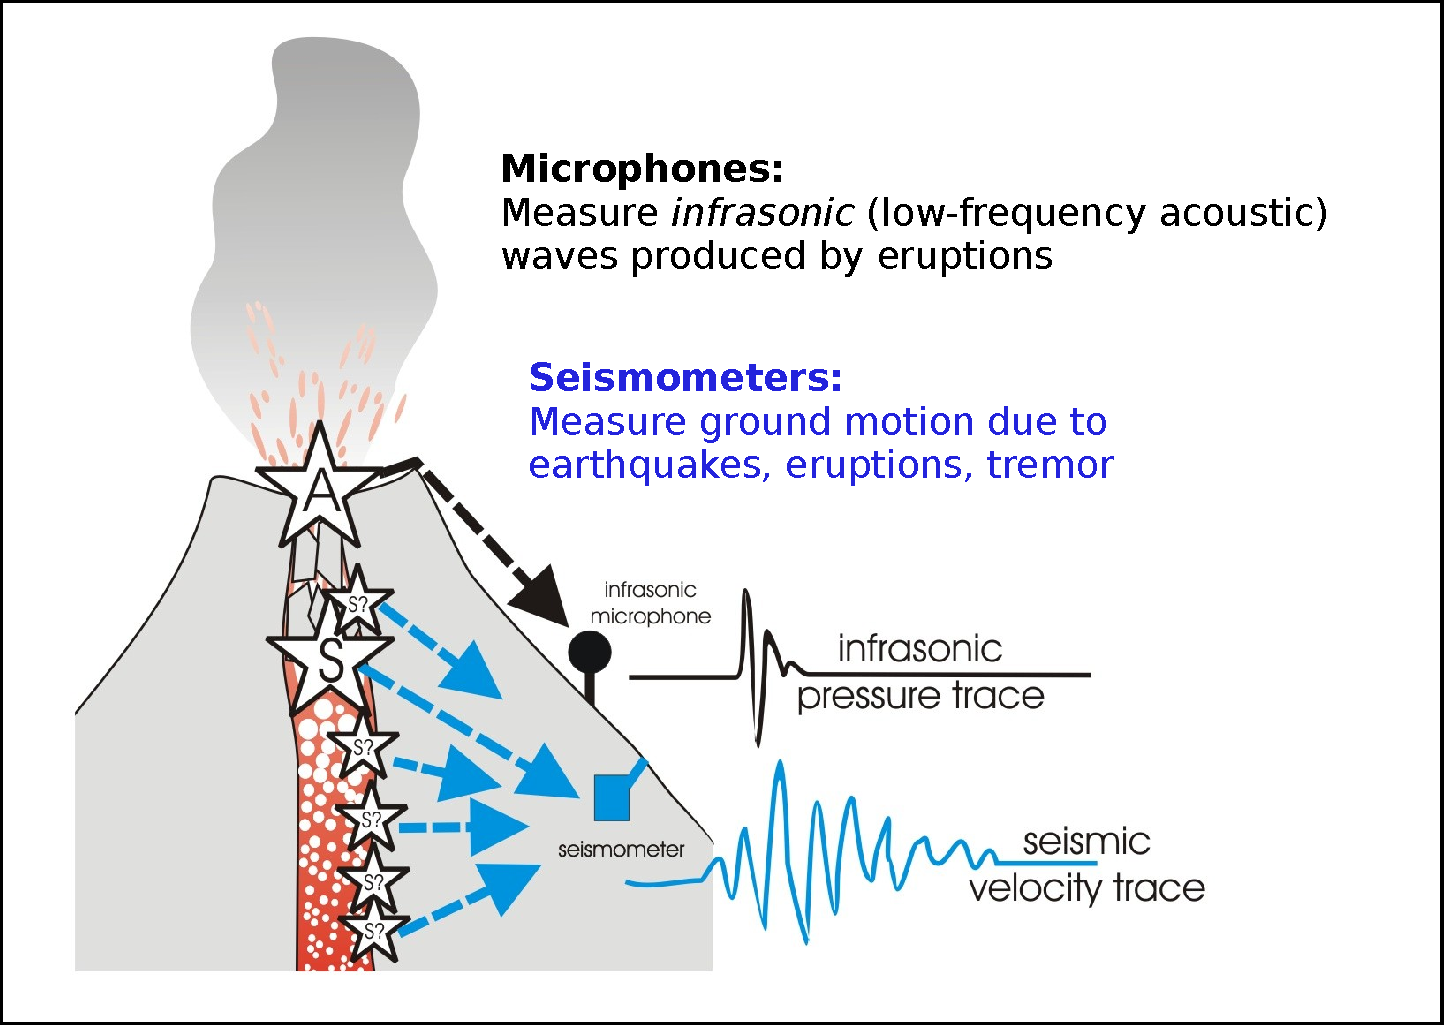
\includegraphics[width=0.9\hsize]{./2-related/figs/NewCartoon.pdf}
\end{center}
\caption{\textbf{Sensors used for volcano monitoring.}}
\label{introduction-fig-cartoon}
\end{figure}

Volcanic monitoring has a wide range of goals related to both scientific
studies and hazard monitoring. Figure~\ref{introduction-fig-cartoon} displays
commonly-used sensors and the signals that they collect. The type and
configuration of the instrumentation deployed depends on the goals of each
study. Traditionally, dispersed networks of seismographs, which record
ground-propagating elastic energy, are used to locate, determine the size of,
and assess focal mechanisms (source motions) of earthquakes occurring within
a volcanic edifice~\cite{Chouet03}. At least four spatially-distributed
seismographs are required to constrain the hypocentral (3D) source location
and origin time of an earthquake, though using more seismic elements enhances
hypocenter resolution and the understanding of source mechanisms.
Understanding spatial and temporal changes in the character of volcanic
earthquakes is essential for tracking volcanic activity and predicting
eruptions and paroxysmal events~\cite{McNutt96}.

\vfill\eject

Another use of seismic networks is imaging the internal structure of a
volcano through tomographic inversion. Earthquakes recorded by
spatially-distributed seismometers provide information about propagation
velocities between a particular source and receiver. A seismically-active
volcano thus allows for three-dimensional imaging of the volcano's velocity
structure~\cite{Benz96,Phillips91}. The velocity structure can then be
related to material properties of the volcano, which may be used to determine
the existence of a magma chamber~\cite{Lees89,Moran99}. Dense array
configurations, with as many as several dozen seismographs, are also an
important focus of volcanic research~\cite{Dietel89,Neuberg94}. Correlated
seismic body and surface wave phases can be tracked as they cross the array
elements, enabling particle motion and wavefield analysis, source
back-azimuth calculations, and enhanced signal-to-noise recovery.

\subsection{Scientific Requirements}

The geophysics community has well-established tools and techniques to process
the signals extracted by volcanic data collection networks. These analytical
methods require that our wireless sensor network provide data of extremely
high fidelity. A single missed or corrupted sample can invalidate an entire
portion of data. Small differences in sampling rates between two nodes can
frustrate analysis. Samples must be accurately time-stamped to allow
comparisons between nodes and between networks.

An important feature of volcanic signals is that much of the data analysis
focuses on discrete events: eruptions, earthquakes, or tremors. While
volcanoes differ significantly in the nature of their activity, during our
2005 Reventador deployment many interesting signals spanned fewer than 60
seconds and occurred at the rate of several dozen per day. This allowed us to
design a network capturing time-limited events, rather than continuous
signals. This is not to say that recording discrete events can answer all the
scientific questions volcanologists pose. Indeed, understanding long-term
trends requires waveforms spanning long time intervals. However, the low
bandwidth of wireless sensor nodes makes them inappropriate for these kinds
of studies, and so we have focused on triggered event collection.

\subsection{Existing Volcano Instrumentation}

\begin{figure}[t]
\begin{center}
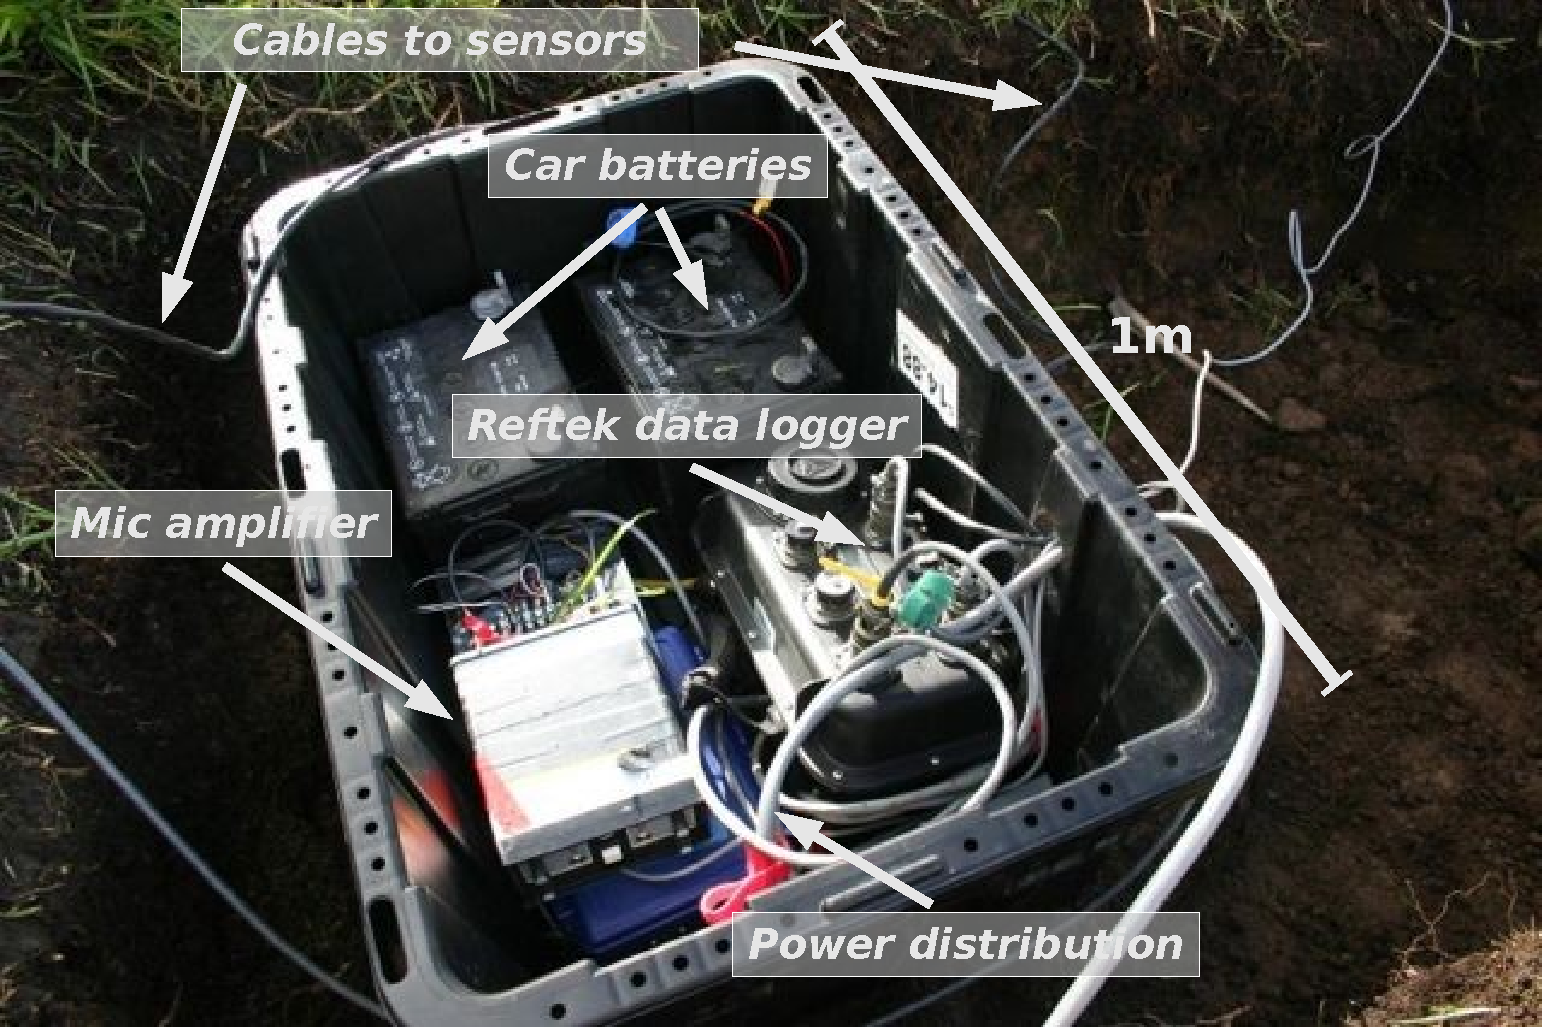
\includegraphics[width=1.0\hsize]{./2-related/figs/Standalone.pdf}
\end{center}
\caption{\textbf{Wired seismoacoustic monitoring station.}}
\label{related-fig-standalone}
\end{figure}

The type of instrumentation used to study volcanoes depends on deployment's
science goals. Geophysicists often use standalone data loggers (e.g., Reftek
130--01~\cite{reftek}) that record signals from seismometers and microphones
to a flash drive. These data loggers are expensive ($\sim$\$9,000), bulky
(8500~$\mathrm{cm}^3$), heavy (2~kg), and power-hungry (1--2.1W), typically
powered by lead-acid car batteries (14.5~kg each) charged by large
(1~$\mathrm{m}^2$) solar panels. The size and weight of the resulting set of
equipment precludes deployments of more than a small number of stations in
remote or hazardous areas.

Figure~\ref{related-fig-standalone} shows an example deployed wired
monitoring station with labeled components. The station shown would support
several high-resolution powered seismometers, acoustic microphones, and other
sensors. The power supply (two lead-acid car batteries), Reftek data logger
with Flash drive to store collected data, signal amplification and power
distribution components are stored together in a large container and buried
underground. The sensors --- in this case, powered seismometers and
microphones --- are deployed nearby with wired connections to the Reftek data
logger. A solar panel may also be located nearby to recharge the car
batteries and enable long-term operation.

\vfill\eject

Typical types of sensing instruments include seismic (see
Figure~\ref{introduction-fig-equipment}~(b) and (c)), acoustic, GPS,
tilt-meter, optical thermal, and gas flux. Volcanic sensors range from widely
dispersed networks to more confined arrays. An individual sensor station
could consist of a single sensor (e.g., seismometer or tilt sensor), or an
array of several closely-spaced ($10^2$ to $10^3$~m aperture) wired sensors,
perhaps of different types. Multiple stations may be integrated into a larger
network installed over an extended azimuthal distribution and radial distance
($10^2$ to $10^4$~m) from the volcanic vent. Data from various stations may
be either recorded continuously or as triggered events and the acquisition
bandwidth depends upon the specific data stream. For instance, seismic data
is often acquired at 24-bit resolution at 100~Hz, while tilt data may be
recorded with 12-bit resolution at 1~Hz or less.

Analog or digital radio telemetry can enable real-time transmission of data
back to an observatory, and is typically installed for monitoring stations
intended to be permanent. However, existing telemetry equipment is bulky and
difficult to install, and its limited radio bandwidth can preclude collecting
large amounts of data from multiple channels.

As a result, many short-duration scientific experiments use a stand-alone
data acquisition system at each recording station. The digitizer performs
high-resolution analog-to-digital conversion from the wired sensors and
stores data on a hard drive or Compact Flash card. However, these systems
require data to be manually retrieved from the station prior to processing,
which can be difficult or time-consuming depending on the location of the
station and the duration of the intended deployment. Depending on the size of
the recording media and number of sensors installed, a station may record
several days or weeks worth of data before it must be serviced.

\vfill\eject

\begin{figure}[t]
\begin{center}
\begin{tabular}{ccc}
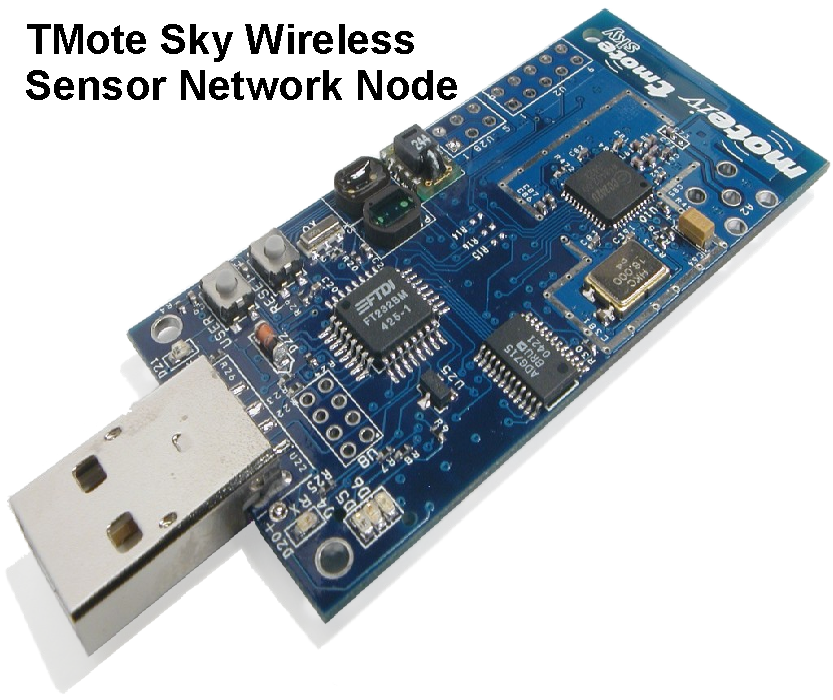
\includegraphics[width=0.3\hsize]{./2-related/figs/TMoteSky.pdf} &
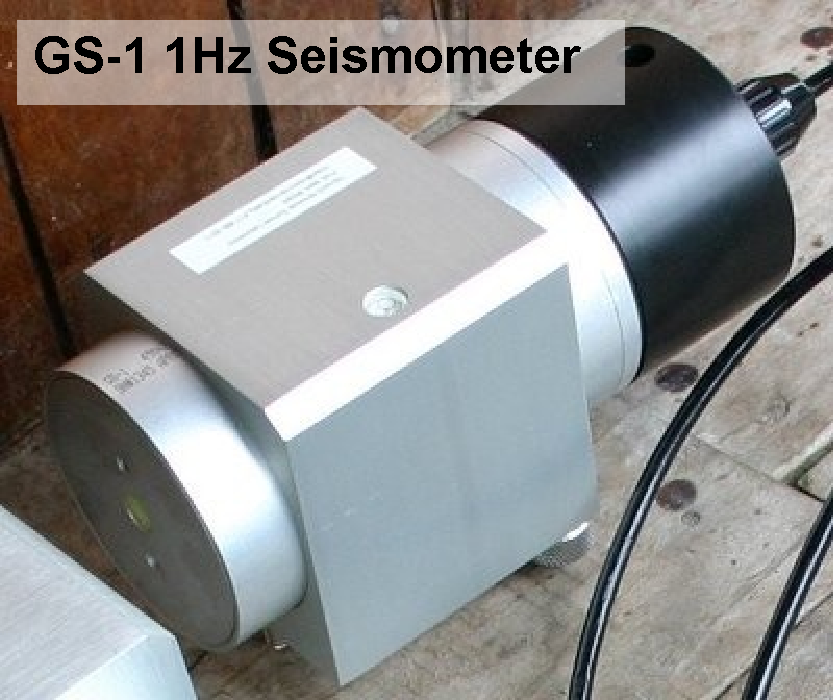
\includegraphics[width=0.3\hsize]{./2-related/figs/GS1.pdf} &
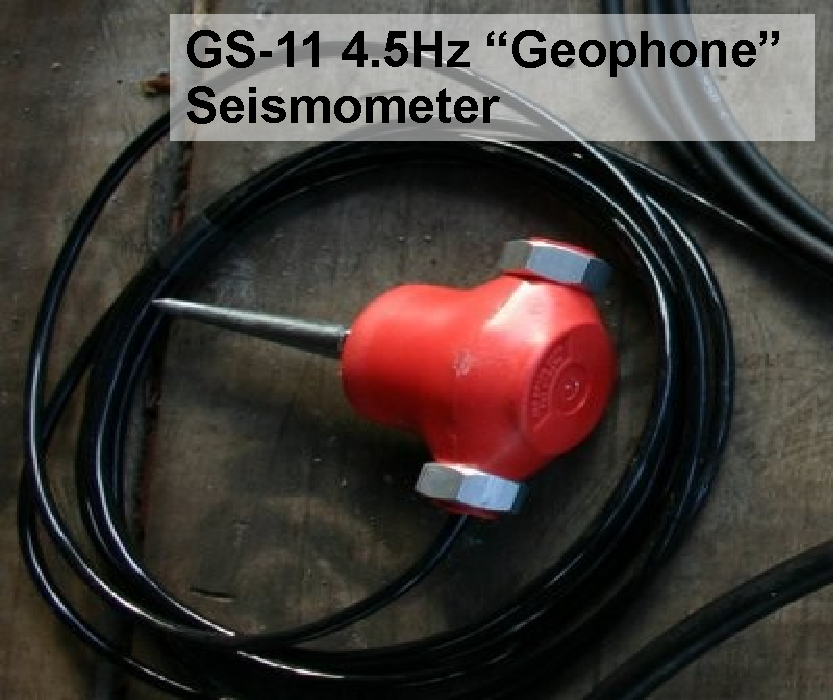
\includegraphics[width=0.3\hsize]{./2-related/figs/GS11.pdf} \\
\textbf{(a)} & \textbf{(b)} & \textbf{(c)} \\
\end{tabular}
\end{center}

\caption{\textbf{Equipment used by our volcano monitoring sensor network.}
From left to right: (a) a TMote Sky sensor ``mote''; (b) a GS-1 1Hz
seismometer; (c) a GS-11 4.5Hz seismometer, or ``Geophone''. Both
seismometers are passive, single-axis instruments. The GS-1 is significantly
more expensive and accurate. Our deployments have used primarily GS-11's, due
to their lower cost.}

\label{introduction-fig-equipment}
\end{figure}

\vspace*{0.05in}

\subsection{Opportunities and Challenges for Sensor Networks}

The number of deployed sensors at a given volcano is usually limited by a
variety of factors, including monetary expenses such as sensor,
communication, and power costs; logistical concerns related to time and
access issues; and archival and telemetry bandwidth constraints. Due to their
small size (12.8~$\mathrm{cm}^3$), light weight (0.015~kg without battery),
low power consumption ($\sim$60~mW) and relatively low cost (\$79), wireless
sensor nodes such as the TMote Sky (see
Figure~\ref{introduction-fig-equipment}~(a)) have an important role to play
in augmenting and extending existing seismic instrumentation, providing the
increased spatial resolution necessary to support applications like
tomography.

Wireless sensor networks have the potential to greatly enhance understanding
of volcanic processes by permitting large deployments of sensors in remote
areas. The science requirements produce unique challenges for sensor
networks, including:

\vfill\eject

\begin{itemize}

\item \textbf{High-resolution signal collection.} Data from seismometers and
microphones must be recorded at relatively high data-rates with adequate
per-sample resolution. A sampling rate of 100~Hz and resolution of 24~bits is
typical. This is in contrast to environmental monitoring sensor networks
targeting low-rate data collection~\cite{gdi-sensys04,berkeley-redwoods}.

\item \textbf{Triggered data acquisition.} Due to limited radio bandwidth it
is infeasible to continuously transmit the full-resolution signal. Instead,
we perform triggered data collection that downloads signals following a
significant earthquake or eruption. This requires sensor nodes to
continuously sample data and detect events of interest. Event reports from
multiple nodes are used to accurately detect well-correlated events.

\item \textbf{Timing accuracy.} To facilitate comparisons of signals across
nodes, signals must be timestamped with an accuracy of one sample time (i.e.,
10~ms at 100~Hz). While data loggers generally incorporate GPS receivers and
low-drift oscillators to maintain accurate timing, equipping each sensor node
with GPS would greatly increase power consumption and cost. Instead, we rely
on a network time synchronization protocol~\cite{rbs,ftsp} and a
\textit{single} GPS receiver. However, correcting for errors in the time
synchronization protocol required extensive post-processing of the raw
timestamps.

\item \textbf{Estimating data quality.} Coping with bandwidth and energy
limitations led us to develop approaches relying on domain-specific notions
of \textit{data quality}. Estimating the inherent \textit{value} of signals
allows us to prioritize resource usage and devote energy and bandwidth to the
most interesting signals. However, our attempts to develop a quality measure
were complicated by the continuous-recording capability of wired data
loggers. Because they are used to working with complete signals spanning long
time intervals, our collaborators were unable to predict how the data loss
due to resource limitations would affect their scientific outcomes.

The interaction between the quality of the signals used and the resulting
scientific conclusions is beyond the scope of this dissertation and not a
problem that we have explored directly. What we have observed is that volcano
scientists begin their studies by interacting with the raw data in
unstructured ways: browsing, zooming in and out, mapping signals between the
time and frequency domains, etc. This type of human-aided data exploration is
not the kind of intelligence we anticipate being able to program into the
network itself. Instead, our preliminary estimates of data quality are based
on established metrics used by the seismology community, which were both easy
to compute and acceptable to our collaborators. Further improving the
estimation of data quality by identifying exactly what data scientists want,
perhaps by using iterative interaction with human experts, is an area of
future work.

\end{itemize}
\clearpage
